\subsection{示例代码}
实现一个简单的可用鼠标或注视(Fuse)操作的小场景。

\emph{HTML}
\begin{lstlisting}[language=HTML]
<a-scene>
  <a-entity
    id="box" cursor="fuse:true;fuseTimeout:1000"
    geometry="primitive: box"
    material="color: blue">
    <a-box
      src="img/logo.jpg"
      position="0 3 -5"
      rotation="45 0 45"
      scale="2 2 2"
      id="box1">
      <a-animation
        attribute="position"
        begin="focus"
        to="0 2.2 -5"
        direction="normal"
        dur="2000">
      </a-animation>
    </a-box>
  </a-entity>

  <a-camera>
    <a-cursor></a-cursor>
  </a-camera>

  <a-plane 
    position="0 0 -4" 
    rotation="-90 0 0" 
    width="4" 
    height="4" 
    color="#7BC8A4">
  </a-plane>
  <a-sky color="#ECECEC"></a-sky>
</a-scene>
\end{lstlisting} 

\emph{JavaScript}
\begin{lstlisting}{language=JavaScript}
document.querySelector('#box')
  .addEventListener('click', function(e) {
    document.querySelector('#box1').emit('focus')
  })
\end{lstlisting}

\subsection{系统截图}
全景漫游系统使用过程中的截图。

\begin{figure}[htp]
\centering
\fbox{
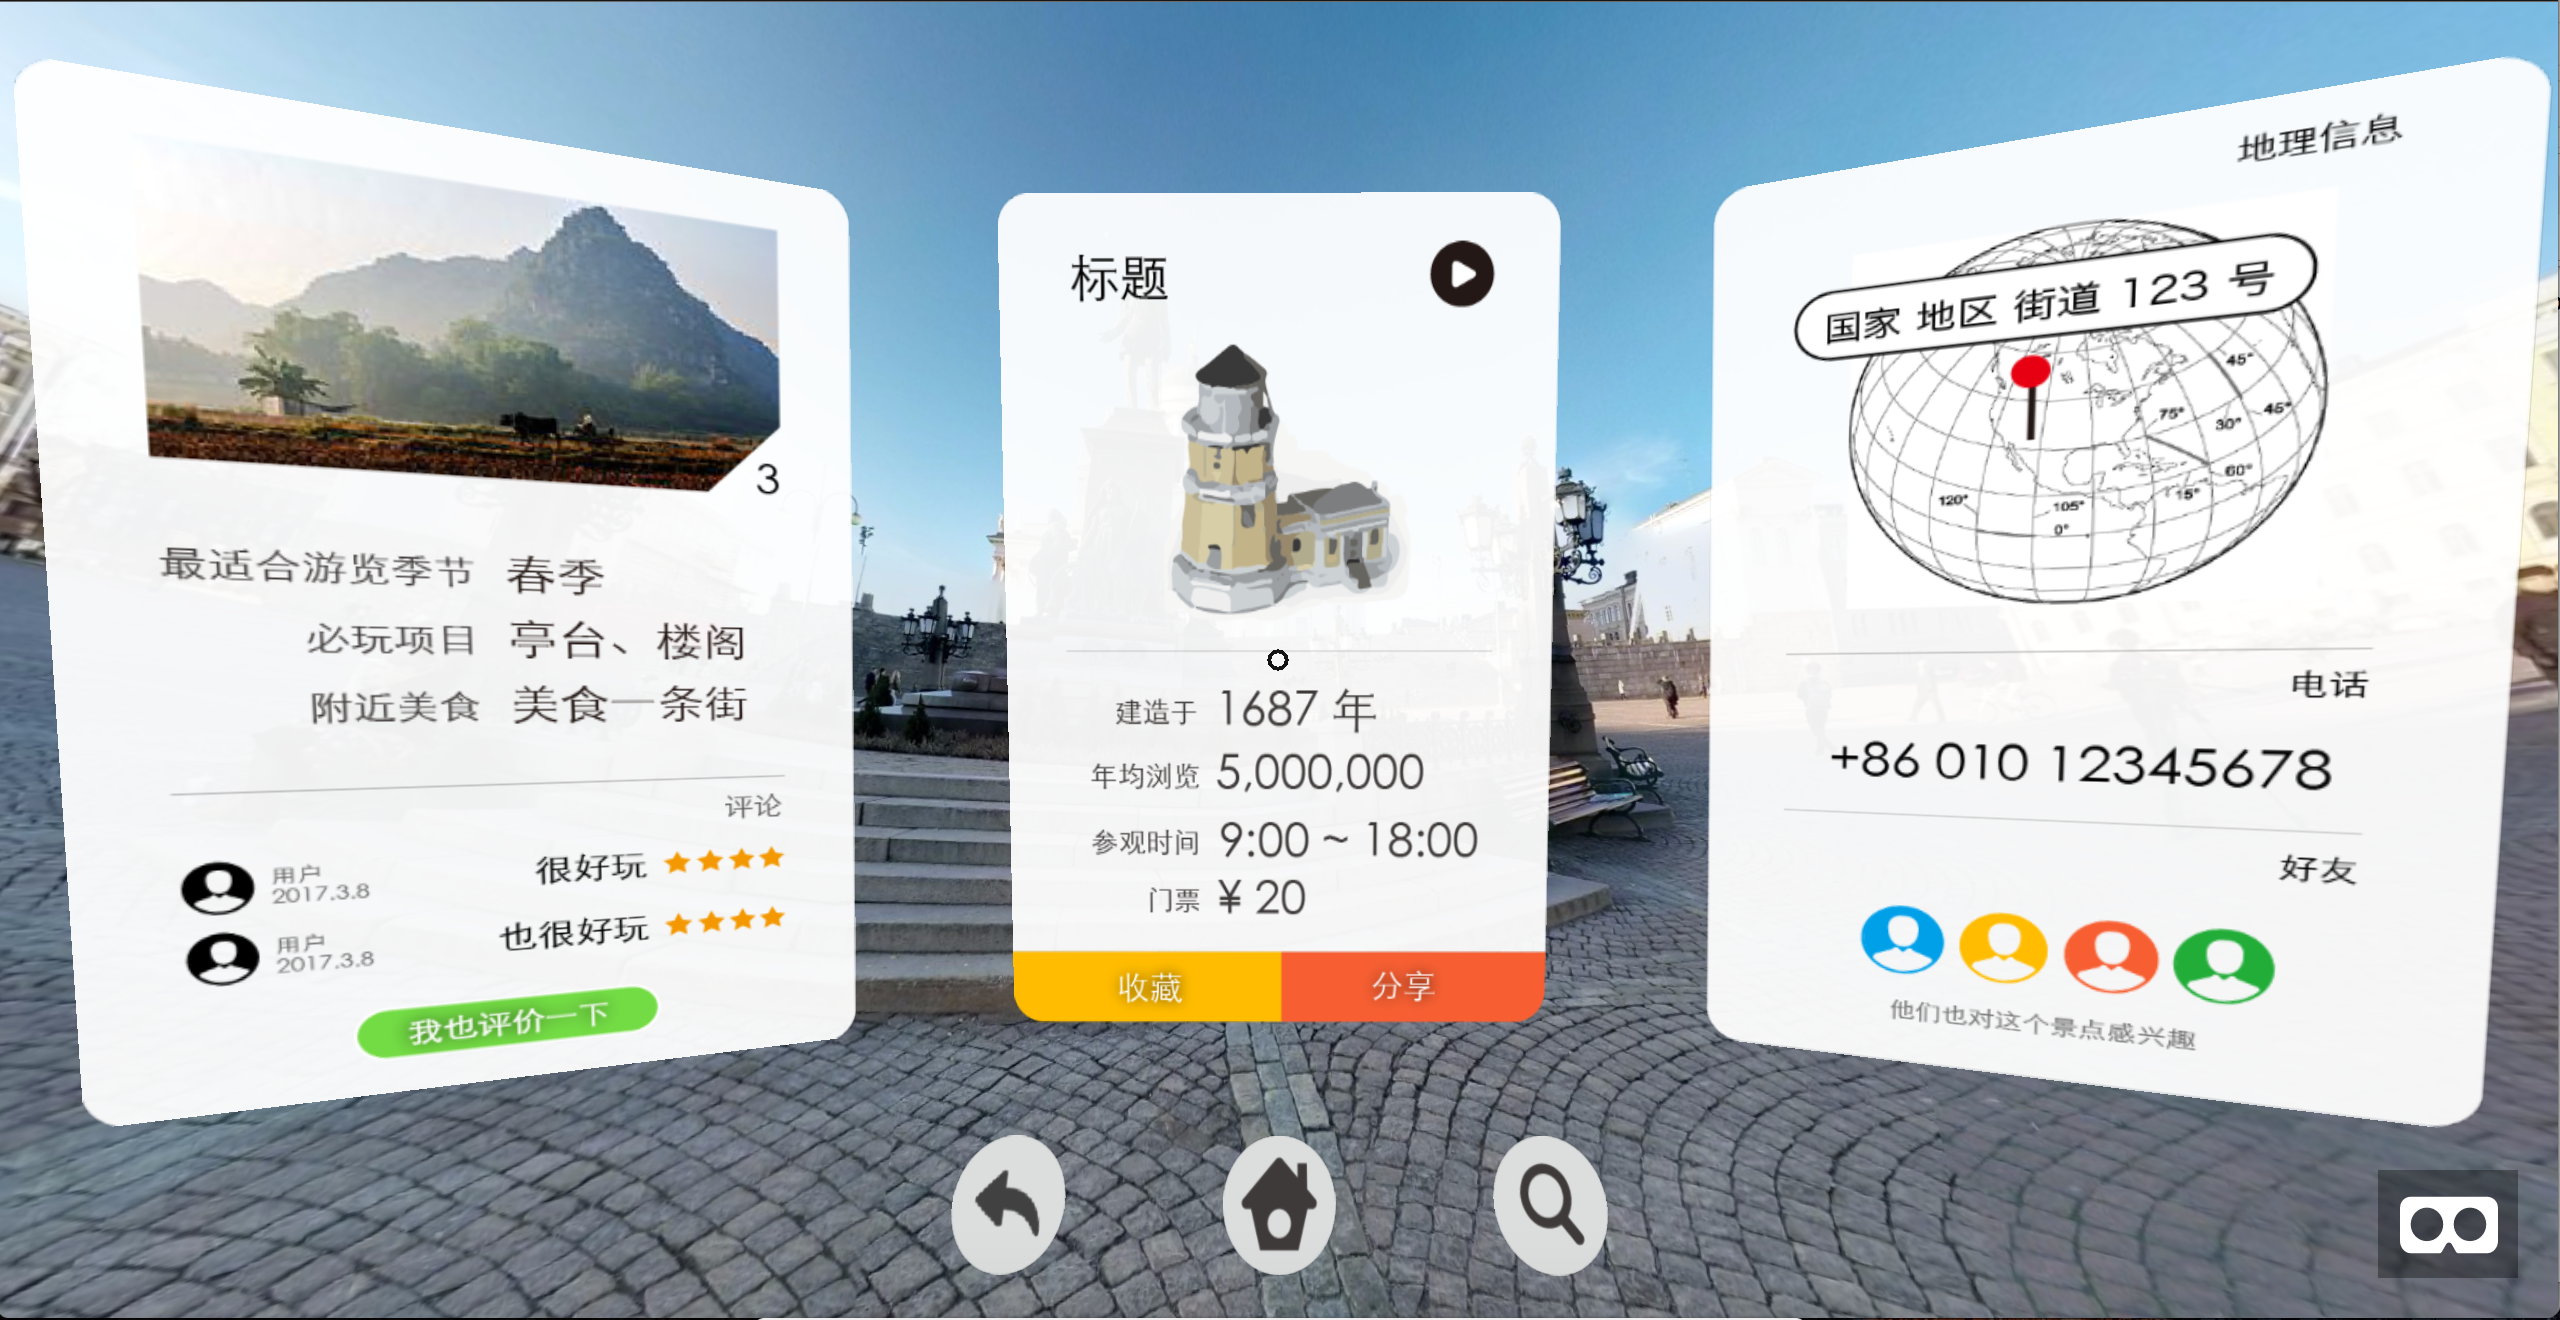
\includegraphics[width=.7\textwidth]{app1}
}
\caption{场景详情界面截图}
\label{fig:app1}
\end{figure}

\begin{figure}[htp]
\centering
\fbox{
\includegraphics[width=.7\textwidth]{app4}
}
\caption{场景分类界面截图}
\label{fig:app4}
\end{figure}

\begin{figure}[htp]
\centering
\fbox{
\includegraphics[width=.7\textwidth]{app2}
}
\caption{支付界面截图}
\label{fig:app2}
\end{figure}

\begin{figure}[htp]
\centering
\fbox{
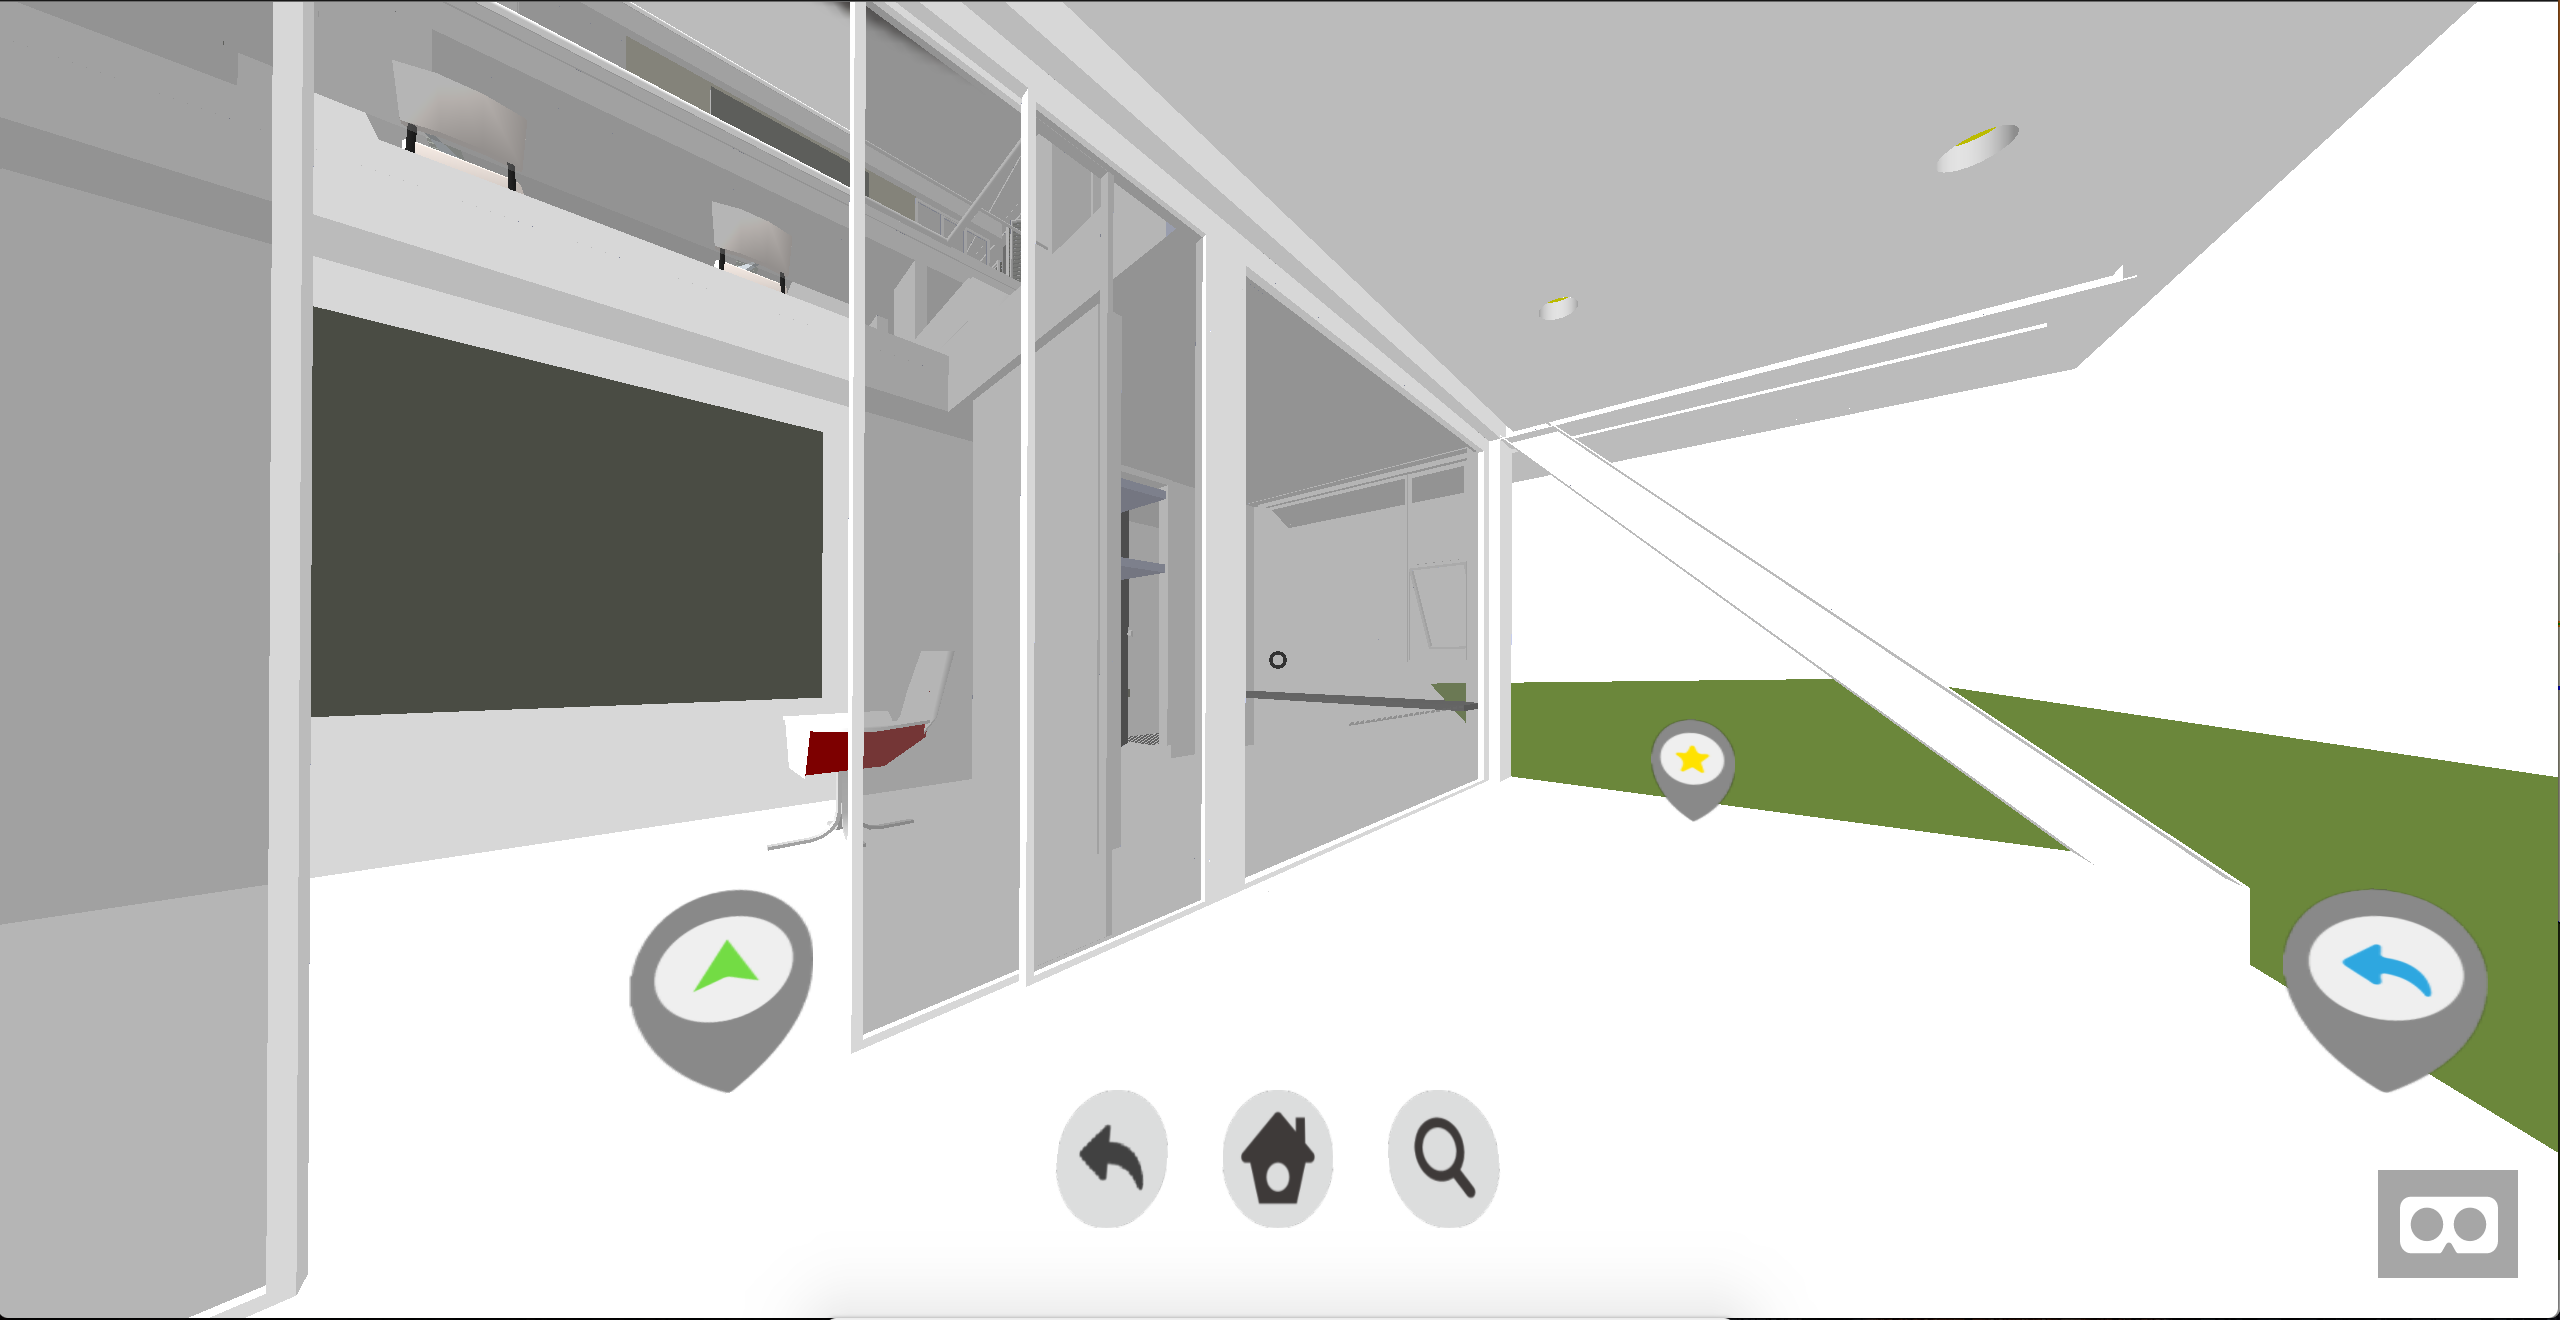
\includegraphics[width=.7\textwidth]{app3}
}
\caption{场景漫游界面截图}
\label{fig:app3}
\end{figure}